\documentclass[a4paper]{article}
\usepackage{microtype}
\usepackage{url,xspace,epsfig,etoolbox}
\usepackage{natbib}
\usepackage{fullpage}
\usepackage[font=bf]{caption}
\usepackage{mdwlist}
\usepackage{graphicx}
\usepackage{wrapfig}

% No page numbers
\pagestyle{empty}

% Use 'Arial' font
\usepackage{helvet}
\renewcommand{\familydefault}{\sfdefault}

% Allow point-size specification of font
\usepackage{fix-cm}

% Allow setting margins on the abstract
\usepackage{changepage}

\newcommand{\projecttitle}{Culture-narration games: a definition and pilot study}

% Prevent indentation of new paragraphs
\setlength{\parindent}{0pt}

% Put space after each paragraph. Note that this matches section titles too,
% and the workaround is below.
\setlength{\parskip}{\baselineskip}

% Allow easy overriding of section and subsection commands
\usepackage{titlesec}
\titleformat{\section}{\bfseries\fontsize{12}{14.4}\selectfont}{}{0em}{}
\titleformat{\subsection}{\bfseries\fontsize{11}{13.2}\selectfont}{}{0em}{}

% No blank line after section titles.
\titlespacing{\section}{0pt}{0pt}{-\baselineskip}
\titlespacing{\subsection}{0pt}{0pt}{-\baselineskip}

% No blank spaces between references
\setlength{\bibsep}{0pt}

% Hanging indent of 0.5 inches in references
\setlength{\bibhang}{0.5in}

% Allow for bigger figures not on their own pages.
% http://tex.stackexchange.com/questions/68516/avoid-that-figure-gets-its-own-page
\renewcommand{\floatpagefraction}{.8}

% Is this blind or not?
\newtoggle{blind}
\toggletrue{blind}

\begin{document}

% Title is bold, centered, 14pt.
% Standard baseline skip is 1.2*fontsize, or 16.8 here.
\begin{center}
\fontsize{14}{16.8}\selectfont
\bf \projecttitle
\end{center}

% Gleaning author placement information from the existing proceedings.
\vspace{-0.25in}
\begin{center}
\iftoggle{blind}{
 % Nothing here: skip authors for blind review
}{
Paul Gestwicki, Kaley Rittichier, and Austin DeArmond, Ball State University\\
pvgestwicki@bsu.edu, kjrittichier@bsu.edu, ajdearmond@bsu.edu\\
}
\end{center}

\newcommand{\totan}{\textit{TotAN}}
\newcommand{\smersh}{\textit{SMERSH}}
\newcommand{\figwidth}{2.5in}

% Abstract: 150 words or less, extra 0.5in left and right margin.
% Note that all text is justified.
%
\begin{adjustwidth}{0.5in}{0.5in}
  \textbf{Abstract:} We are inspired by the educational potential of
  the board game \textit{Tales of the Arabian Nights}, a
  popular game based on the eponymous folk tale. Considering this game
  and others like it, we identify the characteristics that define a
  genre of \textit{culture-narration games}, which we consider to have
  untapped potential for educational and transformative games.
  We describe a design experiment through which a multidisciplinary team
  followed an iterative and incremental process, in collaboration
  with a community partner, to investigate the potential of this genre.
  The result is a game that uses a theme of monsters from around the
  world to teach cultural empathy.
  This pilot project reveals both the promise and several complications
  with the genre, which lead to recommendations for future work.
\end{adjustwidth}

\section{Introduction}


\textit{Tales of the Arabian Nights}~\citep{Goldberg2009} is a 
tabletop board game based on the eponymous folk tale. It was
originally published in 1985~\citep{Goldberg1985}, and it was
re-released with many revisions in 2009.
It is popular among board game hobbyists:
on Board Game Geek, it has a rank of~239 (thematic rank~75),
and Shut Up \& Sit Down rank it as the ninth best game of all 
time~\citep{ShutUp2015}.
In this game, players control a character within a mythical Arabian
setting, exploring the known world to accumulate Story and
Destiny points. The winner is the player who is able to meet their 
Story and Destiny point goal while having a successful encounter
in Baghdad---the City of Peace. 

An intriguing property of \textit{Tales of the Arabian Nights}~(hereafter, \textit{TotAN}) is that it eschews the conventional wisdom for game design,
that player immersion is dependent upon agency.
In \totan{}, 
players choose a destination without any foreknowledge about
what might be encountered there.
They are told the name of the
encounter---such as angry merchant,  powerful prince, or
elephant's graveyard---and based only on this information,
they must choose a reaction from a set of options; for example, 
table~$A$ permits a choice of grovel, aid, rob, avoid, converse,
attack, court, abduct, or honor.
Another player then reads a corresponding entry from 
the \textit{Book of Tales}---a~300-page tome containing~2600 numbered entries.
Most entries provide introductory text followed by paragraphs
tagged with skills that the active player may choose to use, but the choice
is made without any knowledge of potential consequences.
The reader then narrates the conclusion of the
encounter and informs the player of their rewards, which might include
gaining Story or Destiny points, learning new skills, finding treasures, or
gaining status cards that modify players' options in future encounters.
\totan{} then is hardly a game of skill, where the player with the best tactics
wins the game: viewed through this conventional lens, the game is arbitrary
and imbalanced. However, from its design emerges a fanciful gameplay
experience.
Although it is a competitive board game, 
it is not played to win,
but rather for the enjoyment of emerging narrative,
similar to tabletop roleplaying games~\citep{Grouling2001}
or story games~\citep{Duncan2015}.

This property of \totan{} reflects several characteristics
of its source material---a book that ``changed the world on a scale
unrivalled by any other literary text''~\citep[p.1]{Makdisi2008}.
Like the original stories, \totan{} is a collection of shorter stories
that are sometimes linked together and sometimes not.
The characters in the folk tales are often victims of fate with
very little agency over their own encounters. The games rules follow
cultural norms expressed in the folk tales:
you cannot win while sex-changed or on pilgrimage, and both marriage
and children are great blessings---unless you have an ugly baby,
which is shameful.
Baghdad is the most important city in the world, where your adventure starts
and ends.
Furthermore, many stories in \totan{} come directly from the tales,
such as the Sindbad's escape from the valley of diamonds or Aladdin's
entrapment in a magic cave. 

Playing \totan{}  inspired members of our team to read translations
of the original tales,
particularly  the youth-friendly translation by \citep{Neil1994},
which revealed to us the cleverness of the design
and its elegant dovetailing with the source material.
Indeed, although the game was not explicitly designed as a learning game,
we find it exhibits many of the learning game design principles
established by \citet{Klopfer2009}.
Furthermore, in reading the texts, we recognized that we had already
learned elements of the stories and the culture through playing the game,
although not always consciously or explicitly.
This inspired the following analysis, in which we tease apart the
various elements of \totan{}, considering them from both game design
and learning design points of view, and then share the results of a pilot
project to create a technology-enhanced game within the same genre.

\section{Defining the Genre}

We propose that \totan{} is one of very few published games comprising a genre
of \textit{culture-narration games}. Recognizing that the term ``genre''
can be interpreted in multiple ways, we adopt the perspective established
by \citet{Arsenault2009},
that a genre is ``the codified usage of particular mechanics
and game design patterns to express a range of intended play-experiences.''
We define this genre, then, as having the following characteristics.

\begin{enumerate}
\item \textit{Take place in a believable, consistent setting.} 
 Although the world of \totan{} may be unfamiliar to the player,
 everything in it is representative of the world described in the original
 folk tale.
 This includes the contradictions that add depth and nuance, such as 
 the inconsistent treatment of outsiders that emerged from the 
 complex historical roots of the folk tales themselves~\citep{Matar2008}.

\item \textit{Use narrative as a primary feedback mechanism.} 
 In \totan{}, the player's reaction and skill choice yields two forms
 of feedback: the narrative description followed by the changes to the
 game state. The narrative is primary---temporally, visually, and aesthetically.

\item \textit{Have measurable goals.} There is a winning condition as part
 of the social contract of play, following colloquially-accepted 
 standards for board games. The ``game'' is not simply constrained
 cooperative storytelling or a role-playing experience without formal end
 conditions. 

\item \textit{Incorporate endogenously-meaningful ambiguous decisions.}
 Following \citet{Burgun2012}, the decisions that one makes in the game
 are meaningful even though they are made without complete knowledge
 of the game state. For example, a player makes 
 the choice of reaction in \totan{} in hopes that it leads toward skills
 that they have, such as choosing ``Fight'' while in possession of the
 ``Weapon Use'' skill, even though one does not know whether or not
 this skill will have relevance in the resulting entry from the
 \textit{Book of Tales}.

\item \textit{Reward players for decisions that reflects
    cultural understanding.}  The knowledge that a player brings to
  bear on decisions is not just knowledge of in-game systems. 
  A player can predict that choosing to fight a Powerful Ifrit 
 without the Weapon Use skill will not end well,
  but this prediction is not made by having memorized the 
  \textit{Book of Tales}.
  Rather, this prediction draws upon a cultural understanding of power,
  spirits, violence, and much more.
  Note that the game rewards player decisions without resorting to
  clear-cut ``right'' and ``wrong'' (``moral/immoral'',
  ``light side/dark side'', ``paragon/renegade'') choices.  There
  remain unexpected twists: perhaps fighting the Powerful Ifrit without
  combat skills makes him respect you and grant a boon. 
  While the world
  remains consistent, it also embraces the potential for surprising
  results.

\end{enumerate}

Two notable formal elements from \totan{} are intentionally excluded from the
genre definition above. First among these is the oration between players
of each others' stories. While we agree that this is a critical element of 
\totan{}---and that it dovetails performatively 
with Scheherazade's
performances in the source material---it is not clear that this is
characteristic to the genre.  Anecdotal evidence shows that
players with low reading skills can ruin the play experience for other
players, while those players could have read their own stories, aloud or not.
Similarly, \totan{} permits a single-player experience which, while
having a different aesthetic, still seems to produce the same general outcomes
we described above.

The other formal element excluded from the genre definition is the use of an
explicit map. The map is an important tangible aspect of \totan{}, 
in particular with its representation of Baghdad as the largest, most
important city in the world. 
However, we also note that virtual spaces
can be represented without such an explicit map, such as in text adventures,
the MUD family of games, or choose-your-own-adventure books, both of which
use discrete spaces without giving them visual manifestation.

To establish these as characteristics of a genre and not just one game,
we consider another game that possesses them: 
\textit{Agents of SMERSH}~\citep{Maxwell2012}.
\smersh{} is a cooperative game set in the Cold War, with players as 
covert agents trying to stop the entigmatic Dr.\ Lobo---a mad scientist
bent on world domination.
Players move across the world collecting resources and battling henchmen.
While the stories are inspired by spy movies and novels,
the game mechanics are clearly derived from \totan{}: flip a card to read an
encounter title, choose a reaction from a table, hear an introduction,
and then get different results based on skills.
Although \smersh{} uses dice for encounter resolution, the feedback is still
primarily narrative, as illustrated with sample encounters in
Figure~\ref{fig:encounters}.

For contrast, we also consider \textit{Above and Below}~\citep{Laukat2015}, a
worker-management game of city-building.  
%\textit{Above and Below} is primarily about building an
%economic engine that generates victory points faster than your
%opponents within a fixed number of rounds,
Underground exploration includes  player narration
from an encounter book as in \totan{} and \smersh{}, which at first
glance may appear to categorize it as a culture-narration game.
However, in \textit{Above and Below}, reaction choices are thin
wrappers around risk-and-reward balance:
an option is essentially a gamble on being able to roll better
results on the dice, with higher numbers always having better results.
The feedback is primarily in terms of formal rewards, with few
encounters providing any narrative feedback, as illustrated in
the representative encounter of Figure~\ref{fig:encounters}.
Hence, although \textit{Above and Below} includes an encounter book
that players read to each other, it does not satisfy the characteristics
of the culture-narration game genre.

\begin{figure}
\newcommand{\colwidth}{0.48\columnwidth}
% http://tex.stackexchange.com/questions/2441/how-to-add-a-forced-line-break-inside-a-table-cell
\newcommand{\specialcell}[2][t]{%
  \begin{tabular}[#1]{@{}p{\colwidth}@{}}#2\end{tabular}}
\centering
\begin{tabular}{|p{\colwidth}|p{\colwidth}|}\hline
\specialcell{
\\
\totan{} encounter \#1965\\
\\
Many seaside villages have reported sightings and attacks from
a large pirate fleet. There are far too many ships in the fleet to attack
on your own, so you need to find a powerful prince who can stand up to
the pirate captains.\\
\\
\textit{Use Storytelling Skill}\\
\\
You present the plight of the villagers with such eloquence and
style that every prince you address promises to aid in the
defeat of these rampaging pirates. When you see the size of the
fleet sent to destroy the renegades, you have no doubt in the eventual
triumph of justice. [Gain 1 Destiny Point and Courtly Graces skill.]
}
&
\specialcell{
\\
\smersh{} encounter \#20.4.1\\
\\
You have uncovered evidence that UN Agent F9 also works for the CIA.
You're not convinced that's necessarily a bad thing, but the Director
is taking it very seriously. You must find out if he is a threat.\\
\\
You meet with F9 and act as if everything is perfectly normal, exchanging
information about a case you are working together. When he leaves, you follow
him in your Ferrari.\\
\\
\textit{Successfully pass Spycraft test using Driving skill}\\
\\
He is highly experienced at spotting tails, but you are equally experienced
in avoiding being spotted. You follow him to a hotel where he meets
with a Soviet diplomat. Never mind the CIA: it seems he's working for the
KGB. [Improve any two skills.]
}
\\\hline
\specialcell{
\\
\textit{Above and Below} encounter \#62\\
\\
You follow a square tunnel, the walls smooth and masterfully cut.
Before long you reach a tall chamber; in the center sits a great crystal,
floating in mid-air. A dim, violet glow emanates from it and as you approach
a voice fills the air. ``I am the crystal of oracles. If you can prove
your worth, I will give you knowledge.'' Do you continue speaking to the
crystal or explore some of the connecting passages?\\
\\
\textit{Explore the passages}:\\
3 successes: gain two coins\\
5 successes: gain a coin, a fish, and a mushroom
}
& 
\specialcell{
\\
\textit{Traveler's Notebook} encounter\\
\\
As you're sitting on the edge of a river, you see a large turtle swimming towards you. When it gets close it launches from the water to reveal it's not a turtle, but a kappa!\\
\\
\textit{Use Logic skill}\\
\\
Remembering Japanese manners, you give the kappa a greeting bow. It returns your bow, emptying the water-filled dip on its head. It loses its strength and crawls to the water. [Gain 1 Inspiration]
}
\\\hline
\end{tabular}
\caption{Sample encounters}
\label{fig:encounters}
\end{figure}

\section{Cultural Empathy}

We have discussed how \totan{} uses cultural understanding, not only on a
small scale as a way to reward players, but also as a learning outcome of
the game. In order for the game to reward players for their cultural
understanding, cultures must be presented such that they can be understood
by the player. In other words, the game needs to foster a
sense of \textit{cultural empathy}, defining ``empathy'' as 
the ``state of mind in which someone shares the feelings or outlook of
another, sometimes prompted by imaginative exercises 'stepping into
someone's shoes'''~\citep[p.242]{Honderich2005}
Therefore, cultural
empathy, loosely formed, is having empathy for others who are from
different cultures, which allows for better understanding of that
culture.

Cultural empathy is distinct from \textit{cultural
literacy}, which prepares individuals to participate in another culture
based on the information of the culture that they have been 
given~\citep[p.165]{Hirsch1983}. Being culturally literate means having the
ability to participate in another culture that you are
``dropped into,'' similar to how being literate is having the ability to
understand or write a given work of text.  \totan{} focuses on a certain
level of literacy of the given culture. Players are rewarded for their
cultural understanding and their ability to ``perform'' in the given
culture because of the information they have---a form of what
\citet{Travis2011} calls \textit{practomime}.
This is demonstrated in
the example above, understanding the cultural views of marriage and
sex-change have an important role in the game. However, cultural
empathy makes understanding the main point, not
performance. \totan{} relies on an understanding of cultural values as
opposed to just focusing on some of their values consequential
norms. Therefore, though \totan{} expects some sense of cultural
literacy, it focuses more on cultural empathy. When a player walks
away from the game they would not have gained the ability to
participate in a Middle Eastern culture,
although they will have gained some understanding of that culture. 
%This
%is why our emphasis in creating the game has relied more on cultural
%empathy than cultural literacy. We focus more on a mindset of a
%culture, than about facts about the culture. 
Hence, from a learning game design perspective,
cultural empathy is a means to the end of cultural
literacy. However, outside of the game, focusing on cultural literacy
within a semi-fictional world is the means for cultivating
cultural empathy.

\section{Context and Theme}

In order to explore the potentials within this genre,
we formed a team to conduct a design experiment and pilot study.
The team adopted a constructionist perspective~\citep{Papert2001},
that our understanding of the genre would be improved by engaging
with design, development, and evaluation---building prototypes
as a way to understand them.
We formed a partnership with \textit{[omitted for blind review]}, 
a non-lending branch that 
provides community, training, and technology services in a
low socioeconomic area of our city.
The youth patrons of the library tend to be 4rd--6th grade 
``latchkey kids'' who 
see the library as an after-school destination to visit with friends, 
participate in programs, and access technology.

Conversations with program coordinators about culture-narration games
revealed that despite other differences, the youth patrons shared a
fascination with monsters, horror, and the macabre.  This answer in
some ways seemed unsatisfactory: horror and empathy---cultural or
otherwise---do not seem to be a good match. Indeed,
to enjoy horror requires an antithetical dehumanization of its subjects.
However, the love of horror and the monstrous can be
seen throughout our culture, in all forms of media. Indeed, monsters have
been a hook for narratives throughout history. 

\citet{Cohen1996} draws attention to ``reading cultures through the
monsters they engender'' (p.~3).  He notes that the conclusions we
come to about cultures, from monsters or otherwise, will be a
combination of many fragments rather than a ``smooth epistemological
whole.'' A monster is brought about at a particular time and
represents not only the fears prevalent in the culture but also the
values, that lead to that fear (p.~4--12). Pinning that down is
difficult. The monsters work more as a snapshot of the culture at
a particular moment than a definition. This point is especially
important for us to note when creating a game whose goal is to
encourage children's efforts to see something from others'
perspectives.
However, Cohen's theory also helps us understand children's fascination
with monsters, that ``the same creatures who terrify and interdict can evoke potent escapist fantasies''~(p.16).

Our team therefore chose monsters as a key dramatic element for our 
design experiments. They were not only enticing to our target
audience---first observed by our community partner and later proven
through play testing---but Cohen's theory also 
suggests that they also provide an excellent passage for
developing empathy. Monsters represent
various cultures' sameness, in base forms of fear, yet difference, in
the ways that fear becomes specific and embodied. By engendering an
understanding of both difference and sameness between cultures, they
encourage individuals to try to see something from someone else's
viewpoint.


\section{Design Experiment}

Our team comprised ten undergraduate students and one faculty mentor.
The students' majors included Computer Science, English
(Creative Writing), Philosophy, Telecommunications (Audio Production),
and Art (Animation), and 
each earned three credit-hours during a fifteen-week
semester,
working together in a studio space for two hours each Monday, Wednesday,
and Friday.
% In future version, cite the TOCE paper
The team collectively agreed upon three primary goals for the design
experiment in the cultural-narration genre:
to use narrative as the primary form of player feedback;
to teach cultural empathy;
and to use technology to address problems of analog implementations.

The team proceeded with an incremental and
iterative approach to game design and development.
The team used a design log to record design decisions~\citep{Cook2011},
and each iteration
produced an executable release in accordance with best practices of
agile software development~\citep{Cockburn2006};
figures~\ref{fig:screenshots} and~\ref{fig:paper-prototype} demonstrate
artifacts from the design and development process.
Each iteration was tested at
\textit{[the library branch]}, providing valuable feedback to the
team. 
In addition to paper prototypes, the team 
developed software-based prototypes using JavaFX, PlayN, and Polymer, 
all of which allow for HTML5 Web deployment.
Game images and stories were inspired by the team's research on monsters
from world cultures, which included both research sources
(such as \citet{Cohen1996}) and children's books (especially
\citet{Steer2008} and \citet{Stowell2013}).
The team also consulted with local university experts on
games, monsters, world cultures, and literacy.
Each iteration concluded with a retrospective
meeting, which provided an opportunity for the
team's reflective improvement~\citep{Kerth2001,Schon1984}.

\begin{figure}
\centering
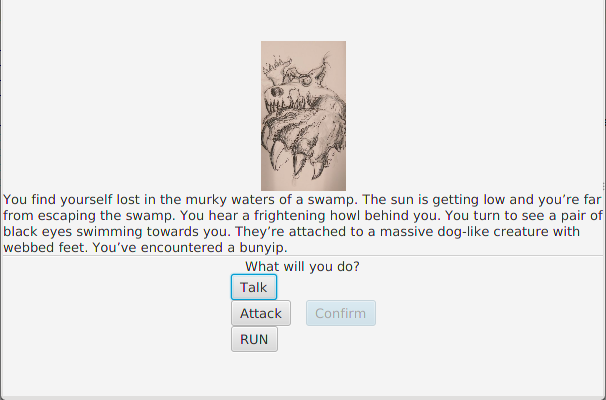
\includegraphics[width=\figwidth]{iteration-1}
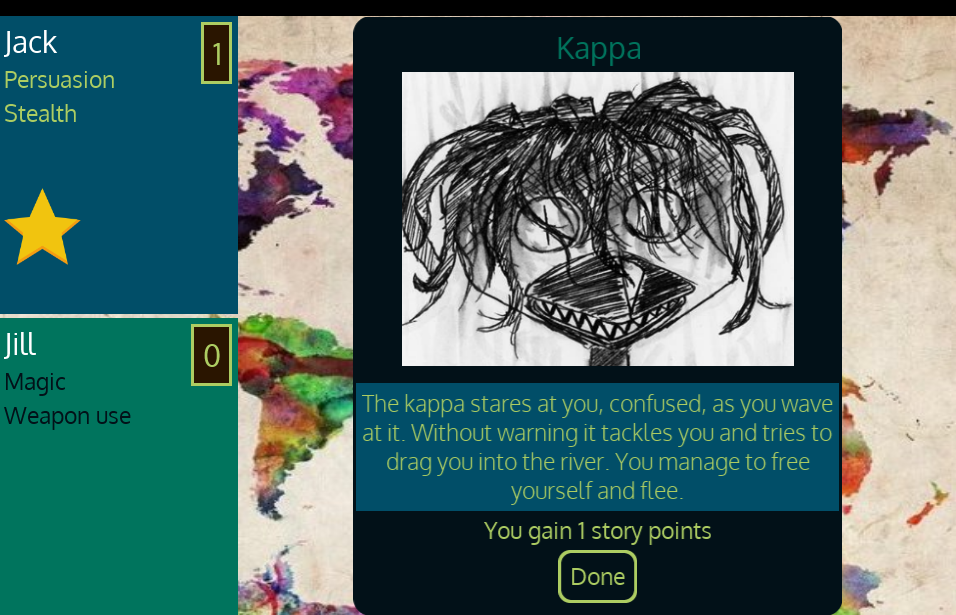
\includegraphics[width=\figwidth]{kappa-encounter}
\caption{Screenshots from Iteration 1 (left) and 2 (right)}
\label{fig:screenshots}
\end{figure}

\begin{figure}
\centering
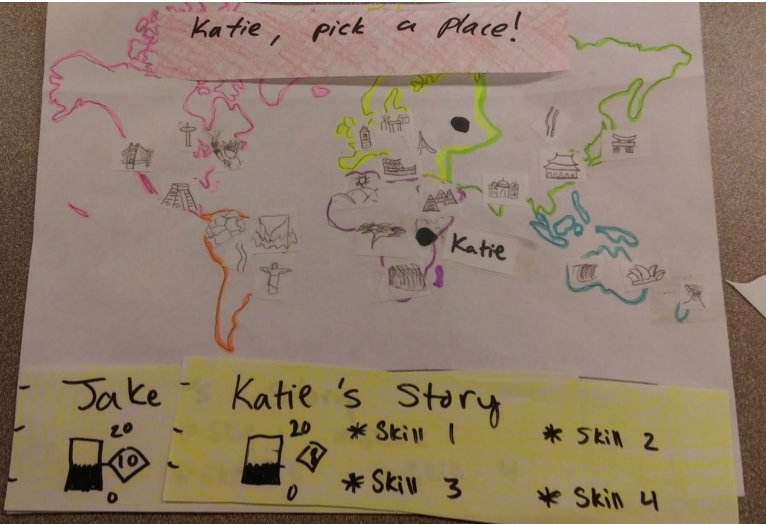
\includegraphics[width=\figwidth]{paper-prototype}
\caption{Paper prototype from Iteration 3}
\label{fig:paper-prototype}
\end{figure}

The title and theme of our game changed between iterations as we came
to a better understanding of the interplay between genre, rules, and our
players.  The final version---\textit{Traveler's Story: Monster
  Tales}---positioned two players as rival authors seeking inspiration
from monsters around the world. The players travel across Africa,
Asia, Europe, Oceania, and North and South America to encounter
monsters from local folklore.  Encounters are patterned after \totan{}
as illustrated in Figure~\ref{fig:encounters}, and the game exhibits
the five characteristics identified for cultural-narration games.

While the visual design and overall rules structure remained stable
throughout the iterations of our experiment, the encounter stories
themselves changed dramatically.
Our target audience required that both stories and gameplay 
had to be much shorter than in other games that we analyzed,
our final version having a 175-character limit.
\textit{[Library branch]} is a high-distraction environment,
where our game competes for attention against both formal and informal
activities. The game takes approximately fifteen minutes to complete,
which we found to be a good balance of keeping players' attention,
making them curious to play again,
and fitting within our limited means for producing content.


\section{Conclusions and Future Work}

Based on our design experiments, pilot study, and understanding of the
literature, we believe there is a significant potential for
culture-narration games as learning tools, particularly for
cultural empathy.
These games combine the educational value of learning from stories
and learning from games, and they provide hooks for designers to 
emphasize various positive skills, including literacy, 
oratory, cultural empathy, history, mathematics, and strategic thinking.
However, as with any educational intervention, these games do not
come without complications.
As others have pointed out~\citep[\textit{e.g.}]{Slota2015}, 
the exact role of narrative in games and in learning is not well
understood. Hence, we focus our conclusions on more immediate
goals of continued fruitful experimentation with culture-narration games.

Physical games such as \totan{} and \smersh{} are expensive to produce
and, for many, intimidating to encounter. \totan{}'s 19-page
instruction booklet may not faze a board game enthusiast, but we have
observed that others are intimidated by the large rulebook, heavy box,
and many components included in the game. Combined with the duration
of play and complexity of rules, such games seem inappropriate for use
in almost all formal educational settings such as conventional
schools.  However, we have found that the combination of technology
enhancement, grade-level writing, and shorter duration circumvents
these problems.  Digital implementations all but eliminate
distribution costs, and with clever game design, children can play the
game in the relatively chaotic environment of an informal after-school
program. With curriculum aides and improved scaffolding, such as
post-game debriefing~\citep{Nicholson2012}
or reflections~\citep{Hickey2013},
we are certain the game could be easily
integrated into school environments, particularly those with
ready access to computers.

The role of text within the game is worthy of particular attention.
The textual expression of narrative requires that players already possess
literacy skills: players who struggle with vocabulary or decoding words
are easily frustrated by such games. There is an opportunity
here as well, to differentiate text based on player reading level
or provide embedded reading aids; however, this also transforms
the outcome of the game from cultural empathy to reading literacy.
Player oration---having players read aloud to each
other---additionally requires oratory skills. We observed engagement
being enhanced when the reader employs theatrical talents as well.
The precise role of oratory skill, self-confidence, and the social
contract of gameplay (the ``magic circle'') is an area for future work.

\section{Acknowledgments}
\textit{The team, organizational, and community partner
  acknowledgments are hidden for blind review.}

\bibliographystyle{apalike}
\bibliography{references}

\end{document} 